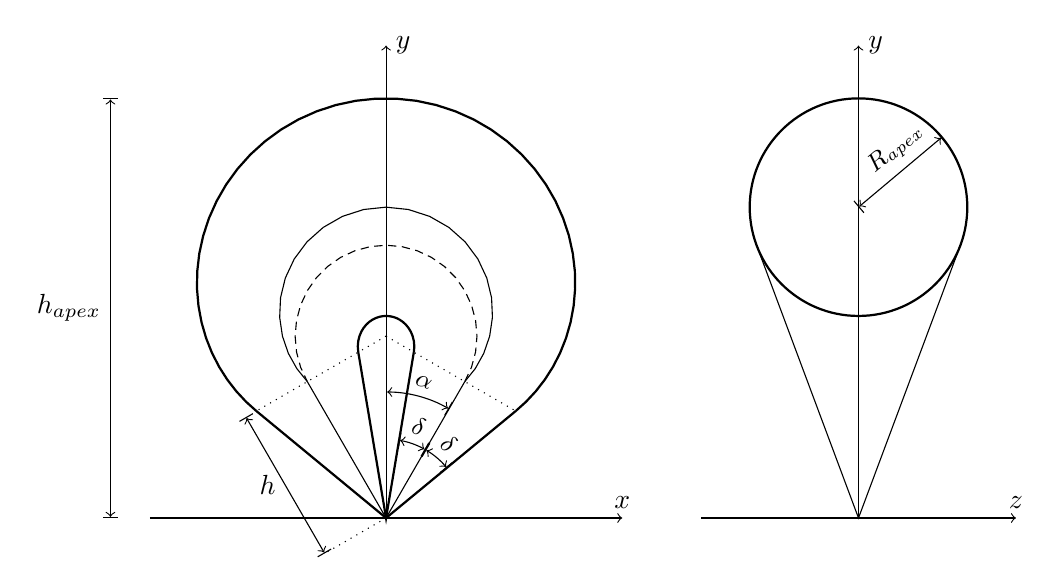
\begin{tikzpicture}
    \def\h{2}
    \def\palpha{30}
    \def\pkappa{0.35}
    
    \def\b{(\h / cos(\palpha))}
    \def\prho{(\h * tan(\palpha))}
    \def\pdelta{asin(\pkappa)}
    
    \def\Xnull{((\prho + \b * \pkappa^2 * sin(\x)) / (1 - \pkappa^2))}
    \def\Rc{sqrt(\Xnull^2 + (\b^2 * \pkappa^2 - \prho^2)/(1 - \pkappa^2))}
    
    \begin{scope}
        % xy view
        \draw[->] (0, 0) -- (0, 6) node[right] {$y$};
        \draw[->] (-3, 0) -- (3, 0) node[above] {$x$};
        
        \draw[densely dashed, domain=-\palpha:180+\palpha] plot ({\prho * cos(\x)}, {\prho * sin(\x) + \b});
        \draw (90+\palpha:\h) -- (0, 0) -- (90-\palpha:\h);
        
        \draw[thick] ({90+\palpha+\pdelta}:{\h/cos(\pdelta)}) -- (0, 0) -- ({90-\palpha-\pdelta}:{\h/cos(\pdelta)});
        \draw[thick] ({90+\palpha-\pdelta}:{\h/cos(\pdelta)}) -- (0, 0) -- ({90-\palpha+\pdelta}:{\h/cos(\pdelta)});
        
        \draw[domain=-\palpha:180+\palpha] plot ({\Xnull * cos(\x)}, {\Xnull * sin(\x) + \b});
        
        \draw[thick,domain=-\palpha:180+\palpha,samples=50] plot ({(\Xnull + \Rc) * cos(\x)}, {(\Xnull + \Rc) * sin(\x) + \b});
        \draw[thick,domain=-\palpha:180+\palpha] plot ({(\Xnull - \Rc) * cos(\x)}, {(\Xnull - \Rc) * sin(\x) + \b});
        
        \draw[dotted] (0, {\b}) -- ({90+\palpha+\pdelta}:{\h/cos(\pdelta)});
        \draw[dotted] (0, {\b}) -- ({90-\palpha-\pdelta}:{\h/cos(\pdelta)});
        
        % definitions of delta, alpha, h and h_apex
        \draw[|<->|] ({90-\palpha-\pdelta}:{\h*0.5}) arc ({90-\palpha-\pdelta}:{90-\palpha}:{\h*0.5}) node[midway, above, rotate={-\palpha - \pdelta/2}] {\small$\delta$};
        \draw[|<->|] ({90-\palpha+\pdelta}:{\h*0.5}) arc ({90-\palpha+\pdelta}:{90-\palpha}:{\h*0.5}) node[midway, above, rotate={-\palpha + \pdelta/2}] {\small$\delta$};
        
        \draw[|<->|] ({90}:{\h*0.8}) arc ({90}:{90-\palpha}:{\h*0.8}) node[midway, above, rotate={-\palpha + \pdelta/2}] {\small$\alpha$};
        
        \def\x{90}
        \draw[|<->|] (0, 0) ++ ({\palpha}:-0.9) -- node[left] {$h$} ++({90+\palpha}:{\h});
        \draw[dotted] (0, 0) -- ++ ({\palpha}:-0.9);
        
        \draw[|<->|] (-3.5, 0) -- node[left] {$h_\text{apex}$} (-3.5, {\b + \Xnull + \Rc});
    \end{scope}
    
    \begin{scope}[xshift=6cm]
        % yz view
        \draw[->] (0, 0) -- (0, 6) node[right] {$y$};
        \draw[->] (-2, 0) -- (2, 0) node[above] {$z$};
        
        % front
        \def\Xnull{((\prho + \b * \pkappa^2 * sin(\x)) / (1 - \pkappa^2))}
        \def\Rc{sqrt(\Xnull^2 + (\b^2 * \pkappa^2 - \prho^2)/(1 - \pkappa^2))}
        \def\x{90}
        
        \draw[thick](0, {\b + \Xnull}) circle (\Rc);
        
        \draw ({90-\pdelta}:{(\b + \Xnull) * cos(\pdelta)}) -- (0, 0) -- ({90+\pdelta}:{(\b + \Xnull) * cos(\pdelta)});
        
        % definition of R_apex
        \draw[|<->|] (0, {\b + \Xnull}) -- node[above,rotate=40,xshift=1.5mm] {\small $R_\text{apex}$} ++ (40:{\Rc});
    \end{scope}
\end{tikzpicture}